\documentclass[a4paper]{article}
\usepackage[14pt]{extsizes} 
\usepackage[T2A]{fontenc}
\usepackage[utf8]{inputenc}
\usepackage{natbib}
\usepackage{graphicx}
\usepackage{amsmath}
\usepackage[english, russian]{babel}
\usepackage{amsmath,amsfonts,amssymb,amsthm,mathtools,mathrsfs}
\usepackage{icomma}
\usepackage{fullpage}
\usepackage{ulem}
\usepackage{eufrak}
\usepackage{setspace}
\usepackage{listings}
\usepackage{indentfirst}
\usepackage[left=2cm,right=1.5cm,top=2cm,bottom=2cm]{geometry}
\usepackage{xcolor}
\usepackage{float}
\usepackage{csquotes}

\setlength{\parindent}{5ex}
\setlength{\parskip}{1em}
\renewcommand{\baselinestretch}{1}

\graphicspath{{images/}}

\definecolor{buzzlightyear}{HTML}{8757A5}
\definecolor{grass}{HTML}{738D06}
\definecolor{literal}{HTML}{F18A2B}
\definecolor{commentcolor}{HTML}{8E908B}

\lstdefinestyle{habrstyle}{
    backgroundcolor=\color{white},   
    commentstyle=\color{commentcolor},
    keywordstyle=\bfseries\color{buzzlightyear},
    numberstyle=\tiny\color{commentcolor},
    stringstyle=\color{grass},
    basicstyle=\ttfamily\footnotesize,
    breakatwhitespace=false,         
    breaklines=true,                 
    captionpos=b,                    
    keepspaces=true,                 
    numbers=left,                    
    numbersep=5pt,                  
    showspaces=false,                
    showstringspaces=false,
    showtabs=false,                  
    tabsize=4
}

\lstset{style=habrstyle}

\begin{document}
    % НАЧАЛО ТИТУЛЬНОГО ЛИСТА
    \begin{center}
        \begin{center}
        \hfill \break
        \normalsize{Санкт-Петербургский государственный политехнический}\\
        \normalsize{университет Петра Великого}\\
        \hfill \break
        \normalsize{\textbf{Высшая школа интеллектуальных систем и}}\\ 
        \normalsize{\textbf{суперкомпьютерных технологий}}\\ 
        \hfill \break
        \hfill \break
        \hfill \break
        \normalsize{Лабораторная работа №9}\\
        \hfill \break
        \hfill \break
        \normalsize{\LARGE Дифференцирование и интегрирование}\\
        \end{center}
        \hfill \break
        \hfill \break
        \hfill \break
        \hfill \break
        \hfill \break
        \hfill \break
        \hfill \break
        \hfill \break
        \hfill \break
        \hfill \break
        \begin{flushright}
            \normalsize{Выполнил студент 3-го курса}\\
            \normalsize{группа 3530901/80201}\\
            \normalsize{Матвеец Андрей Вадимович}\\
            \hfill \break
            \normalsize{Преподаватель:}\\
            \normalsize{Богач Наталья Владимировна}\\
        \end{flushright}
        \hfill \break
        \hfill \break
        \hfill \break
        \hfill \break
        \begin{center} Санкт-Петербург\end{center}
        \begin{center}2021\end{center} 
        \thispagestyle{empty}
    \end{center}
    % КОНЕЦ ТИТУЛЬНОГО ЛИСТА
    
    % ОГЛАВЛЕНИЕ
    \newpage
        \tableofcontents
    
    % СПИСОК ИЛЛЮСТРАЦИЙ
    \newpage
         \listoffigures
    
    % СПИСОК ЛИСТИНГОВ     
    \newpage
         \lstlistoflistings   
     
    \newpage
        \section{Часть №1: \texttt{chap09.ipynb}}
            В первой части лабораторной работы нам необходимо запустить все примеры из \texttt{chap09.ipynb}, прочитать все описания, после чего заменить пилообразный сигнал на входе на непериодические данные \texttt{Facebook}, после чего повторно запустить все примеры.
            
            Начнем с загрузки непериодических данных \texttt{Facebook} и представления их в виде графика:
            
            \begin{figure}[H]
                \centering
                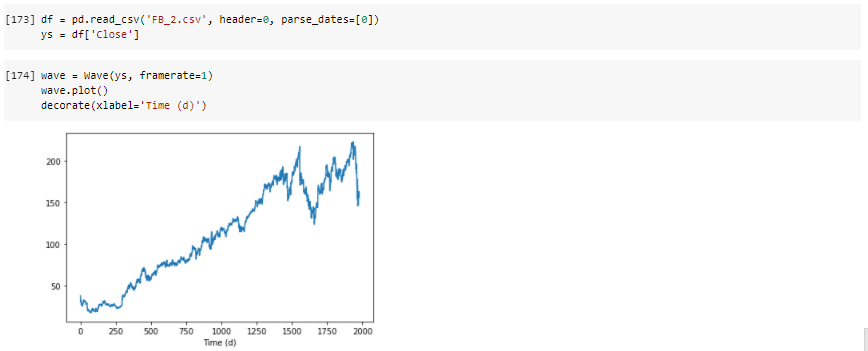
\includegraphics[width=\textwidth]{ex_1_new_wave.png}
                \caption{Непериодические данные \texttt{Facebook}}
                \label{fig:ex_1_new_wave}
            \end{figure}
            
            После этого посмотрим на спектр полученных данных:
            
            \begin{figure}[H]
                \centering
                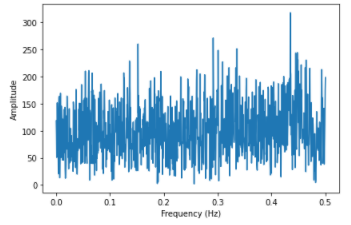
\includegraphics{ex_1_new_spectr.png}
                \caption{Спектр данных \texttt{Facebook}}
                \label{fig:ex_1_new_spectr}
            \end{figure}
            
            Теперь, из-за того, что между гармониками входные компоненты маленькие, установим эти отношения на NaN и посмотрим на результат:
            
\begin{lstlisting}[language=Python, caption= \texttt{Ratio spectrum}]
    ratio_spectrum = out_spectrum.ratio(in_spectrum, thresh=1)
    ratio_spectrum.plot(marker='.', ms=4, ls='')
    
    decorate(xlabel='Frequency (Hz)',
             ylabel='Amplitude ratio',
             yscale='log')
\end{lstlisting}
            
            \begin{figure}[H]
                \centering
                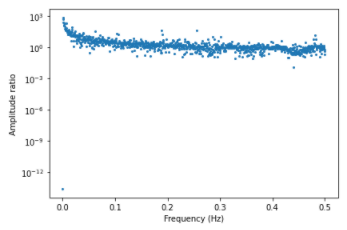
\includegraphics{ex_1_new_ratio_spectr.png}
                \caption{Полученные результаты}
                \label{fig:ex_1_new_ratio_spectr}
            \end{figure}
            
            После этого сравним вычисленные отношения с фильтром. Сразу можно заметить, что данные не совпадают, идет большой разброс:
            
\begin{lstlisting}[language=Python, caption= Сравнение вычисленного отношения с фильтром]
    cumsum_filter.plot(label='cumsum filter')
    ratio_spectrum.plot(label='ratio', marker='.', ms=4, ls='')
    decorate(xlabel='Frequency (Hz)',
             ylabel='Amplitude ratio',
             yscale='log')
\end{lstlisting}
            
            \begin{figure}[H]
                \centering
                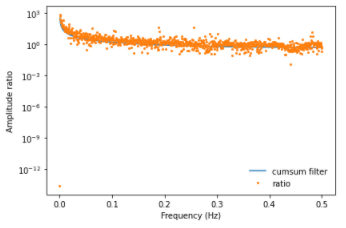
\includegraphics{ex_1_new_custom_filret.png}
                \caption{Результаты сравнения вычисленного отношения с фильтром}
                \label{fig:ex_1_new_custom_filret}
            \end{figure}
            
            Наконец, сравним полученные результаты с входными:
            
\begin{lstlisting}[language=Python, caption= Сравнение вычисленного отношения с фильтром]
    out_wave.plot(label='summed', alpha=0.7)

    cumsum_filter.hs[0] = 0
    out_wave2 = (in_spectrum * cumsum_filter).make_wave()
    out_wave2.plot(label='filtered', alpha=0.7)
    
    decorate(xlabel='Time (s)')
\end{lstlisting}
            
            \begin{figure}[H]
                \centering
                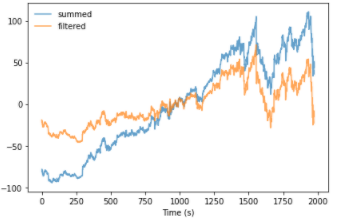
\includegraphics{ex_1_new_result.png}
                \caption{Итоговое сравнение}
                \label{fig:ex_1_new_result}
            \end{figure}
            
            Как видно в итоговом сравнении, полученные графики не равны.
            
    \newpage
        \section{Часть №2: \texttt{diff} и \texttt{differentiate}}
            Во втором пункте лабораторной работы нам необходимо изучить влияние \texttt{diff} и \texttt{differentiate} на сигнал. Для этого необходимо создать треугольный сигнал, распечатать его и применить к нему \texttt{diff}. Затем вычислить спектр треугольного сигнала, применить \texttt{differentiate} и потом напечатать результат. 
            
            Начнем с создания треугольного сигнала и сразу же выведем его на экран:
            
\begin{lstlisting}[language=Python, caption= Создание и вывод треугольного сигнала]
    in_wave = TriangleSignal(freq=50).make_wave(duration=0.1, framerate=44100)
    in_wave.plot()
    decorate(xlabel='Time (s)')
\end{lstlisting}
            
            \begin{figure}[H]
                \centering
                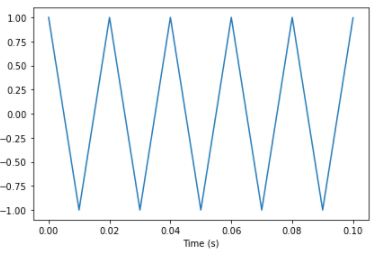
\includegraphics{ex_2_1.png}
                \caption{Треугольный сигнал}
                \label{fig:ex_2_1}
            \end{figure}
            
            Теперь применим \texttt{diff} и выведем полученный график:
            
\begin{lstlisting}[language=Python, caption= Применение \texttt{diff}]
    out_wave = in_wave.diff()
    out_wave.plot()
    decorate(xlabel='Time (s)')
\end{lstlisting}
            
            \begin{figure}[H]
                \centering
                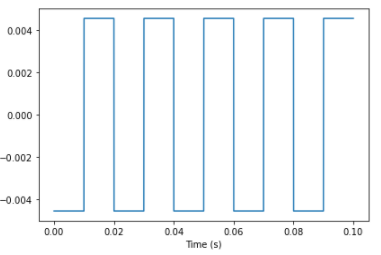
\includegraphics{ex_2_2.png}
                \caption{Применение \texttt{diff}}
                \label{fig:ex_2_2}
            \end{figure}
            
            Как видно - \texttt{diff} треугольной волны - прямоугольная волна.
            
            Теперь вычислим спектр и применим к нему \texttt{differentiate}
            
\begin{lstlisting}[language=Python, caption= Вычисление спектра и применение \texttt{differentiate}]
    out_wave2 = in_wave.make_spectrum().differentiate().make_wave()
    out_wave2.plot()
    decorate(xlabel='Time (s)')
\end{lstlisting}
            
            \begin{figure}[H]
                \centering
                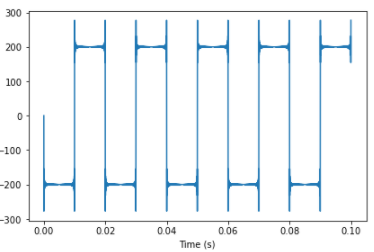
\includegraphics{ex_2_3.png}
                \caption{Применение \texttt{differentiate}}
                \label{fig:ex_2_3}
            \end{figure}
            
            На графике виден необычный эффект. Он вызван тем, что производная треугольной волны не определена в точках "треугольника".
            
    \newpage
        \section{Часть №3: \texttt{cumsum} и \texttt{integrate}}
            В третьем пункте лабораторной работы нам необходимо изучить влияние \texttt{cumsum} и \texttt{integrate} на сигнал. Для этого необходимо создать прямоугольный сигнал, распечатать его и применить к нему \texttt{cumsum}. Затем вычислить спектр треугольного сигнала, применить \texttt{integrate} и потом напечатать результат. 
            
            Начнем с создания прямоугольного сигнала и сразу распечатаем его:
            
\begin{lstlisting}[language=Python, caption= Создание и вывод прямоугольного сигнала]
    in_wave = SquareSignal(freq=50).make_wave(duration=0.1, framerate=44100)
    in_wave.plot()
    decorate(xlabel='Time (s)')
\end{lstlisting}
            
            \begin{figure}[H]
                \centering
                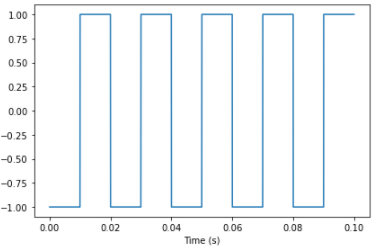
\includegraphics{ex_3_1.png}
                \caption{Прямоугольный сигнал}
                \label{fig:ex_3_1}
            \end{figure}
            
            Теперь применим к полученному сигналу \texttt{cumsum} и выведем полученный график:
            
\begin{lstlisting}[language=Python, caption= Применение \texttt{cumsum}]
    out_wave = in_wave.cumsum()
    out_wave.plot()
    decorate(xlabel='Time (s)')
\end{lstlisting}
            
            \begin{figure}[H]
                \centering
                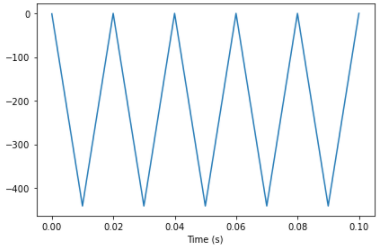
\includegraphics{ex_3_2.png}
                \caption{Применение \texttt{cumsum}}
                \label{fig:ex_3_2}
            \end{figure}
            
            Как видно - \texttt{cumsum} для прямоугольной волны - треугольная волна.
            
            Кроме того спектральный интеграл так же является треугольной волной:
            
\begin{lstlisting}[language=Python, caption= Применение \texttt{integrate}]
    spectrum = in_wave.make_spectrum().integrate()
    spectrum.hs[0] = 0
    out_wave2 = spectrum.make_wave()
    out_wave2.plot()
    decorate(xlabel='Time (s)')
\end{lstlisting}
            
            \begin{figure}[H]
                \centering
                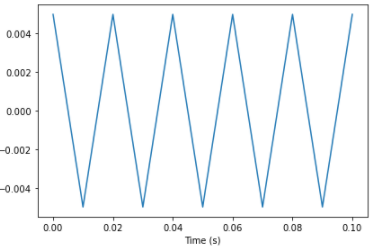
\includegraphics{ex_3_3.png}
                \caption{Применение \texttt{integrate}}
                \label{fig:ex_3_3}
            \end{figure}
            
            Доказать схожесть сигналов можно сместив и нормализовав обе волны:
            
\begin{lstlisting}[language=Python, caption= Смещение и нормализация сигналов]
    out_wave.unbias()
    out_wave.normalize()
    out_wave2.normalize()
    out_wave.plot()
    out_wave2.plot()
\end{lstlisting}
            
            \begin{figure}[H]
                \centering
                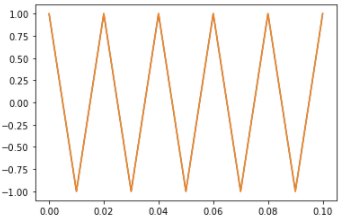
\includegraphics{ex_3_4.png}
                \caption{Результат смещения и нормализации сигналов}
                \label{fig:ex_3_4}
            \end{figure}
            
            Для того, чтобы точно определить насколько полученные графики схожи напишем следующую строчку:

            \begin{figure}[H]
                \centering
                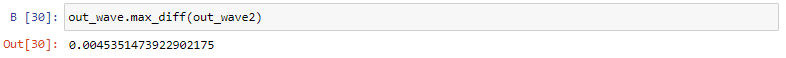
\includegraphics[width=\textwidth]{ex_3_5.png}
                \caption{Результат сравнения}
                \label{fig:ex_3_5}
            \end{figure}
            
            По результатам видно, что различия в сигналах почти неразличимы.
            
    \newpage
        \section{Часть №4: Двойное интегрирование}
            В четвертом пункте лабораторной работы нам необходимо изучить влияние двойного интегрирования. Для этого надо создать пилообразный сигнал, вычислить его спектр и дважды применить \texttt{integrate}, после чего напечатать результирующий сигнал, и его спектр.
            
            Начнем с создания пилообразного сигнала и сразу распечатаем его:
            
\begin{lstlisting}[language=Python, caption= Создание и вывод пилообразнного сигнала]
    in_wave = SawtoothSignal(freq=50).make_wave(duration=0.1, framerate=44100)
    in_wave.plot()
    decorate(xlabel='Time (s)')
\end{lstlisting}
            
            \begin{figure}[H]
                \centering
                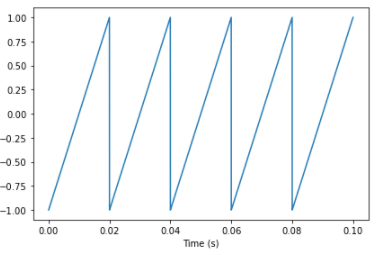
\includegraphics{ex_4_1.png}
                \caption{Пилообразный сигнал}
                \label{fig:ex_4_1}
            \end{figure}
            
            Теперь применим к полученному сигналу \texttt{cumsum} и выведем полученный график:
            
\begin{lstlisting}[language=Python, caption= Применение \texttt{cumsum}]
    out_wave = in_wave.cumsum()
    out_wave.unbias()
    out_wave.plot()
    decorate(xlabel='Time (s)')
\end{lstlisting}
            
            \begin{figure}[H]
                \centering
                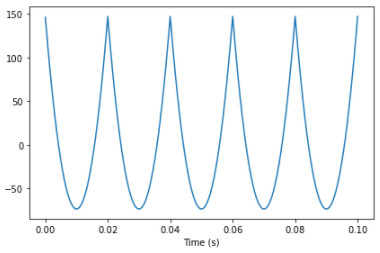
\includegraphics{ex_4_2.png}
                \caption{Применение \texttt{cumsum}}
                \label{fig:ex_4_2}
            \end{figure}
            
            Как видно - первая сумма пилообразного сигнала - парабола.
            
            Опять применим функцию \texttt{cumsum}:
            
\begin{lstlisting}[language=Python, caption= Второе применение \texttt{cumsum}]
    out_wave = out_wave.cumsum()
    out_wave.plot()
    decorate(xlabel='Time (s)')
\end{lstlisting}
            
            \begin{figure}[H]
                \centering
                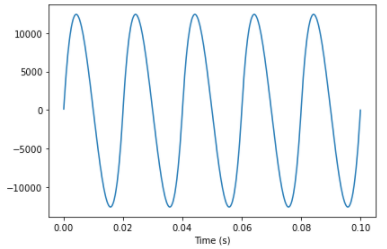
\includegraphics{ex_4_3.png}
                \caption{Второе применение \texttt{cumsum}}
                \label{fig:ex_4_3}
            \end{figure}
            
            Как видно - вторая сумма пилообразного сигнала - кубическая кривая.
            
            Наконец, применим к исходному пилообразному сигналу два раза \texttt{integrate} и посмотрим на результат:
            
\begin{lstlisting}[language=Python, caption= Применение \texttt{integrate}]
    spectrum = in_wave.make_spectrum().integrate().integrate()
    spectrum.hs[0] = 0
    out_wave2 = spectrum.make_wave()
    out_wave2.plot()
    decorate(xlabel='Time (s)')
\end{lstlisting}
            
            \begin{figure}[H]
                \centering
                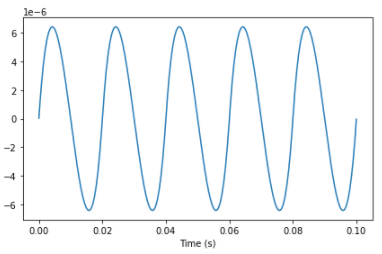
\includegraphics{ex_4_4.png}
                \caption{Применение \texttt{integrate}}
                \label{fig:ex_4_4}
            \end{figure}
            
            Полученный результат так же представлят собой кубическую кривую.
            
            Данный график напоминает синусоиду, так как \texttt{integrate} действует как фильтр НЧ. Для более понятного отображения посмотрим на спектр полученного сигнала:
            
\begin{lstlisting}[language=Python, caption= Применение спектра]
    out_wave2.make_spectrum().plot(high=500)
\end{lstlisting}
            
            \begin{figure}[H]
                \centering
                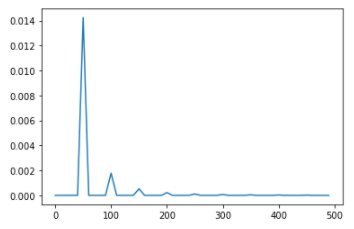
\includegraphics{ex_4_5.png}
                \caption{Полученный спектр}
                \label{fig:ex_4_5}
            \end{figure}
            
            В результате стало понятно, что это график не синусоиды, а именно кубической кривой.
            
    \newpage
        \section{Часть №5: Вторая разность и вторая производная}
            В пятом пункте лабораторной работы нам необходимо изучить влияние второй разности и второй производной. Для этого надо создать \texttt{CubicSignal}, вычислить двойную разность применив \texttt{diff} и проанализировать результат. После этого вычислить вторую производную, дважды применив \texttt{differentiate} к спектру. 
            
            Начнем с создания \texttt{CubicSignal} и сразу выведем его на экран:
            
\begin{lstlisting}[language=Python, caption= Создание и вывод \texttt{CubicSignal}]
    in_wave = CubicSignal(freq=0.0005).make_wave(duration=10000, framerate=1)
    in_wave.plot()
\end{lstlisting}
            
            \begin{figure}[H]
                \centering
                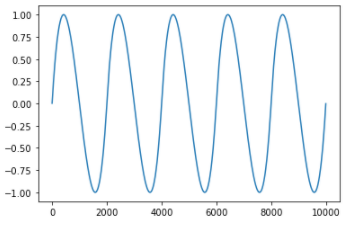
\includegraphics{ex_5_1.png}
                \caption{\texttt{CubicSignal}}
                \label{fig:ex_5_1}
            \end{figure}
            
            Теперь применим к полученному сигналу \texttt{diff} и выведем полученный график:
            
\begin{lstlisting}[language=Python, caption= Применение \texttt{diff}]
    out_wave = in_wave.diff()
    out_wave.plot()
\end{lstlisting}
            
            \begin{figure}[H]
                \centering
                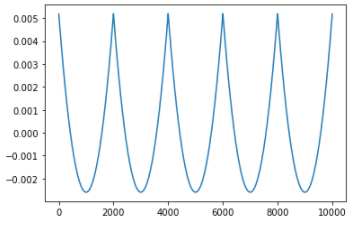
\includegraphics{ex_5_2.png}
                \caption{Применение \texttt{diff}}
                \label{fig:ex_5_2}
            \end{figure}
            
            В результате мы получили параболу.
            
            Опять применим функцию \texttt{diff}:
            
\begin{lstlisting}[language=Python, caption= Второе применение \texttt{diff}]
    out_wave = out_wave.diff()
    out_wave.plot()
\end{lstlisting}
            
            \begin{figure}[H]
                \centering
                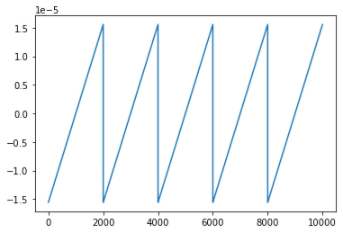
\includegraphics{ex_5_3.png}
                \caption{Второе применение \texttt{diff}}
                \label{fig:ex_5_3}
            \end{figure}
            
            Теперь мы получили пилообразную волну.
            
            После этого применим к исходному пилообразному сигналу два раза \texttt{differentiate} и посмотрим на результат:
            
\begin{lstlisting}[language=Python, caption= Применение \texttt{differentiate}]
    spectrum = in_wave.make_spectrum().differentiate().differentiate()
    out_wave2 = spectrum.make_wave()
    out_wave2.plot()
    decorate(xlabel='Time (s)')
\end{lstlisting}
            
            \begin{figure}[H]
                \centering
                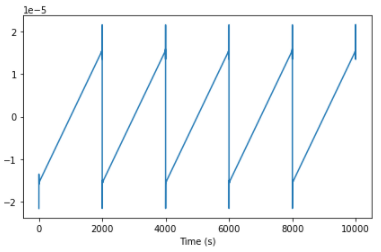
\includegraphics{ex_5_4.png}
                \caption{Применение \texttt{differentiate}}
                \label{fig:ex_5_4}
            \end{figure}
            
            В результате мы получили такой же пилообразный сигнал, но с неким "шумом". Это связано с тем, что производная параболического сигнала не определена в некоторых точках.
            
            Затем найдем нужный фильтр для первой производной:
            
\begin{lstlisting}[language=Python, caption= Нахождение фильтра для первой производной]
    diff_window = np.array([-1.0, 2.0, -1.0])
    padded = zero_pad(diff_window, len(in_wave))
    diff_wave = Wave(padded, framerate=in_wave.framerate)
    diff_filter = diff_wave.make_spectrum()
    diff_filter.plot(label='2nd diff')
    decorate(xlabel='Frequency (Hz)', ylabel='Amplitude ratio')
\end{lstlisting}
            
            \begin{figure}[H]
                \centering
                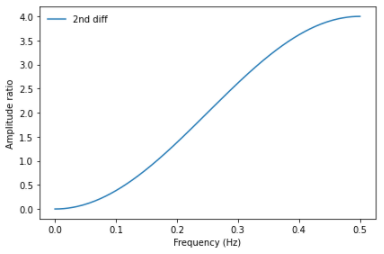
\includegraphics{ex_5_5.png}
                \caption{Нахождение фильтра для первой производной}
                \label{fig:ex_5_5}
            \end{figure}
            
            Чтобы найти фильтр для второй производной нужно возвести фильтр первой производной в квадрат:
            
\begin{lstlisting}[language=Python, caption= Нахождение фильтра для второй производной]
    deriv_filter = in_wave.make_spectrum()
    deriv_filter.hs = (PI2 * 1j * deriv_filter.fs)**2
    deriv_filter.plot(label='2nd deriv')
    decorate(xlabel='Frequency (Hz)', ylabel='Amplitude ratio')
\end{lstlisting}
            
            \begin{figure}[H]
                \centering
                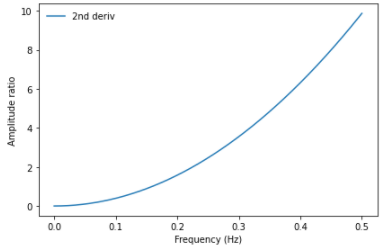
\includegraphics{ex_5_6.png}
                \caption{Нахождение фильтра для второй производной}
                \label{fig:ex_5_6}
            \end{figure}
            
            Полученный фильтр для второй производной является параболическим и поэтому он усиливает самые высокие частоты
            
            Теперь представим оба полученных графика на одном:
            
\begin{lstlisting}[language=Python, caption= Сравнение графиков]
    diff_filter.plot(label='2nd diff')
    deriv_filter.plot(label='2nd deriv')
    decorate(xlabel='Frequency (Hz)', ylabel='Amplitude ratio')
\end{lstlisting}
            
            \begin{figure}[H]
                \centering
                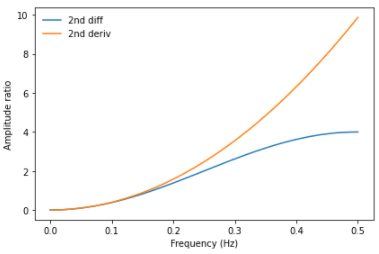
\includegraphics{ex_5_7.png}
                \caption{Сравнение графиков}
                \label{fig:ex_5_7}
            \end{figure}
            
            В результате можно сказать, что оба полученных фильтра являются высокочастотными, которые усиливают компоненты наивысшей частоты. Именно поэтому на низких частотах различий совершенно никаких нет, но они становятся заметными на высоких частотах.
            
    \newpage
        \section{Выводы}
             В результате выполнения лабораторной работы мы научились дифференцировать и интегрировать функции, разобрались с работой \texttt{diff}, \\\texttt{differentiate}, \texttt{cumsum} и \texttt{integrate}. Кроме того, изучили влияние двойного интегрирования, второй разности и второй производной  на разные сигналы.
            
\end{document}
